\documentclass{article}

%other packages
\usepackage[a4paper]{geometry}
\usepackage{longtable}
\usepackage{wrapfig}
\setlength\parindent{0pt}
\usepackage{enumitem}
\usepackage[table,dvipsnames]{xcolor}
\usepackage{polynom}
\def\scaleint#1{\vcenter{\hbox{\scaleto[3ex]{\displaystyle\int}{#1}}}}
\usepackage{array}
\newcolumntype{C}{>{{}}c<{{}}} % for '+' and '-' symbols
\newcolumntype{R}{>{\displaystyle}r} % automatic display-style math mode 
\usepackage{tabularray}
\usepackage{dcolumn,tabularx,booktabs}
\usepackage[most]{tcolorbox}

%maths
\usepackage{mathtools}
\usepackage{amsmath}
\usepackage{amssymb}
\usepackage{amsfonts}
\usepackage{autobreak}

%tikzpicture
\usepackage{tikz}
\usepackage{scalerel}
\usepackage{pict2e}
\usepackage{tkz-euclide}
\usepackage{tikz-3dplot}
\usetikzlibrary{calc}
\usetikzlibrary{patterns,arrows.meta}
\usetikzlibrary{shadows}
\usetikzlibrary{external}
\usetikzlibrary{decorations.pathreplacing,angles,quotes}

%pgfplots
\usepackage{pgfplots}
\pgfplotsset{compat=1.18}
\usepgfplotslibrary{statistics}
\usepgfplotslibrary{fillbetween}

\pgfplotsset{
    standard/.style={
    axis line style = thick,
    trig format=deg,
    enlargelimits,
    axis x line=middle,
    axis y line=middle,
    enlarge x limits=0.15,
    enlarge y limits=0.15,
    every axis x label/.style={at={(current axis.right of origin)},anchor=north west},
    every axis y label/.style={at={(current axis.above origin)},anchor=south east}
    }
}

\begin{document}

Math 115 - Week 6, Class 14 - 5 Feb 2024
\hrule


\vspace{10pt}

We proceeded with the lecture material: Integration by Parts. This follows from the product rule of differentiation - essentially, if we are integrating a product, it lets us simplify one of the functions that is being multiplied (through differentiation). You choose which one to differentiate based on whether the resulting integral becomes easier or not. Recall that the $\int$ sign is basically an operation which recovers something based on its differential.

\begin{align*}
\frac{d}{dx}[uv]&=u\cdot\frac{dv}{dx}+v\cdot\frac{du}{dx}\\
d(uv)&=u\ dv+v\ du\\
u\ dv&=\ d(uv)-v\ du\\
\int u\ dv&=\int\ d(uv)-\int v\ du
\end{align*}

\begin{equation}
\int u\ dv=uv-\int v\ du
\end{equation}

\vspace{10pt}

{\bf{}EXAMPLE} Solve $\displaystyle\int x3^x\ dx$

\vspace{10pt}

Our known methods of substitution don't work here - try them if you want, they only make the integral more complicated. But for this nail, we now have a hammer - Integration by Parts!

\begin{align*}
\int x3^x\ dx&=\left(\begin{aligned}u=x&\quad du=\ dx\\dv=3^x\ dx&\quad v=3^x/\ln3\end{aligned}\right)\\
&=x\frac{3^x}{\ln3}-\int\frac{3^x}{\ln3}\ dx\\
&=\frac{x3^x}{\ln3}-\frac{3^x}{(\ln3)^2}+C
\end{align*}

\begin{center}
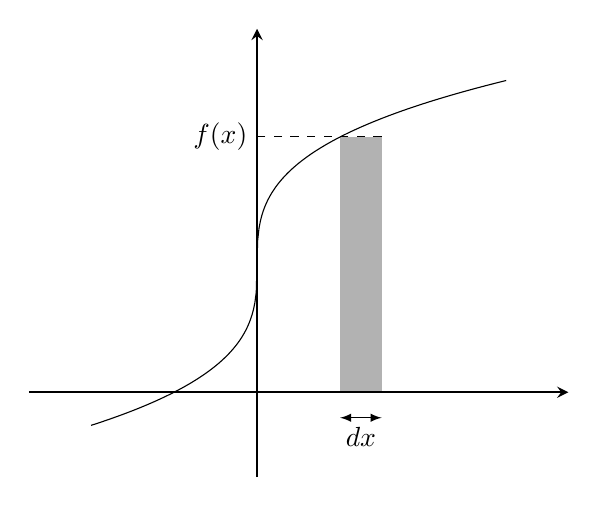
\begin{tikzpicture}
\begin{axis}[
standard,
xtick={\empty}, ytick={\empty},]
\addplot[domain=-2:3,samples=300] {((x)/abs(x))*(abs(x))^(1/3)+1};
\fill[opacity=0.3] (1,0) -- (1,2) -- (1.5,2) -- (1.5,0) -- cycle;
\draw[latex-latex] (1,-0.2) -- (1.5,-0.2) node[pos=0.5,below]{$dx$};
\draw[dashed] (1.5,2) -- (0,2) node[pos=1,left]{$f(x)$};
\end{axis}
\end{tikzpicture}
\end{center}

\vspace{10pt}

This neat little graphic shows how we can derive the area differential from the $x$ differential. That is, $dA=f(x)\ dx$. And we just use the symbol which recovers something from its differential to find the area: $\int\ dA=A=\int f(x)\ dx$.

\vspace{10pt}

{\bf{}EXAMPLE} Evaluate $\displaystyle\int(x^2+3x)\cos2x\ dx$

\vspace{10pt}

When doing Integration by parts, we choose as $u$ the term which becomes simpler upon differentiation. In this case, the polynomial $(x^2+3x)$ fits this bill.

\begin{align*}
\int(x^2+3x)\cos2x\ dx&=\left(\begin{aligned}u=x^2+3x&\quad du=(2x+3)\ dx\\dV=\cos2x\ dx&\quad V=\frac{1}{2}\sin2x\ dx\end{aligned}\right)\\
&=(x^2+3x)\cdot\frac{1}{2}\sin2x-\int\frac{1}{2}\sin(2x)\cdot(2x+3)\ dx\\
&=\frac{1}{2}(x^2+3x)\sin2x-\frac{1}{2}\int(2x+3)\cdot\sin2x\ dx\\
&=\left(\begin{aligned}2x+3=u&\quad2x\ dx=\ du\\\sin2x\ dx=\ dV&\quad\frac{1}{2}\cos2x=V\end{aligned}\right)\\
&=\frac{1}{2}(x^2+3x)\sin2x-\frac{1}{2}\left(-\frac{1}{2}(2x+3)\cos(2x)-\int\left(-\frac{1}{2}\cos(2x)\right)\cdot2\ dx\right)\\
&=\frac{1}{2}(x^2+3x)\sin(2x)+\frac{1}{4}(2x+3)\cos(2x)-\frac{1}{2}\cdot\frac{1}{2}\sin(2x)+C\\
&=\frac{1}{2}(\sin2x)(x^2+3x-\frac{1}{2})+\frac{1}{4}(2x+3)\cos2x+C
\end{align*}

\vspace{10pt}

An alternative to Integration by Parts is Integration by Undetermined Coefficients, but it isn't taught in the course.

\vspace{10pt}

Recall:

\begin{align*}
\color{OliveGreen}\int\cos(ax+b)\ dx&\color{OliveGreen}=\cos(ax)\ d(ax)\cdot\frac{1}{a}\\
&\color{OliveGreen}=\frac{1}{a}\int\cos t\ dt\\
&\color{OliveGreen}=\frac{1}{a}\sin t+C=\frac{1}{a}\sin(ax)+C
\end{align*}

\vspace{10pt}

Likewise,

\begin{align*}
\color{OliveGreen}\int\sin(ax+b)&\color{OliveGreen}=\cdots\\
\color{OliveGreen}\cdots&\color{OliveGreen}=-\frac{1}{a}\cos(ax+b)+C
\end{align*}

\newpage

{\bf{}EXAMPLE} Evaluate $\displaystyle\int\arctan x\ dx$

\begin{align*}
\int\arctan x\ dx&=\left(\begin{aligned}\arctan x=u&\quad du=\frac{1}{1+x^2}\ dx\\dx=\ dv&\quad V=x\end{aligned}\right)\\
&=x\arctan x-\int\frac{x}{1+x^2}\ dx\\
&=\left(\begin{aligned}x^2+1=t\\2x\ dx=\ dt\\x\ dx=\frac{1}{2}\ dt\end{aligned}\right)\\
&=x\arctan x-\frac{1}{2}\int\frac{dt}{t}=x\arctan x-\frac{1}{2}\ln|t|+C\\
&=x\arctan x-\frac{1}{2}\int\frac{dt}{t}=x\arctan x-\frac{1}{2}\ln|x^2+1|+C
\end{align*}

\vspace{10pt}

{\bf{}EXAMPLE} Evaluate $\displaystyle\int5^{x^2+4}\cdot x\ dx$

\begin{align*}
\int5^{x^2+4}\cdot x\ dx&=\left(\begin{aligned}x^2+4=t\\2x\ dx=\ dt\end{aligned}\right)\\
&=\frac{1}{2}\cdot\frac{5^{x^2+4}}{\ln5}+C
\end{align*}

\end{document}